%%%%%%%%%%%%%%%%%%%%%%%%%%%%%%%%%%%%%%%%%%%%%%%%%%%%%%%%%%%%%%%%%%%%%%%%%%%%%%%%%%%%%%%
%	FYP Report 2012 - Lee Wei Yeong (lwy08)	%
%%%%%%%%%%%%%%%%%%%%%%%%%%%%%%%%%%%%%%%%%%%%%%%%%%%%%%%%%%%%%%%%%%%%%%%%%%%%%%%%%%%%%%%
\documentclass{icldt}
\def \supervisor   {Prof. Susan Eisenbach}
\def \secondmarker {Dr. Tristan Allwood}
%%%%%%%%%%%%%%%%%%%%%%%%%%%%%%%%%%%%%%%%%%%%%%%%%%%%%%%%%%%%%%%%%%%%%%%%%%%%%%%%%%%%%%%
\usepackage{amsmath, amssymb, amsthm} % AMS packages
\usepackage{graphicx}                 % graphics and color
\usepackage[usenames,dvipsnames]{color}
\usepackage[T1]{fontenc}              % correct text encoding
\usepackage[utf8]{inputenc}
\usepackage{url}
\usepackage{algorithm, algorithmic}
\usepackage{subfigure}
\usepackage{moreverb}
\usepackage{eukdate}
\usepackage[english,british]{babel}
\usepackage{parskip}				  % justified paragraphs + newlines
\usepackage{minted}
\usepackage{float}
\usepackage{appendix}
\usepackage[svgnames]{xcolor}
\usepackage{fancyvrb}
\usepackage{courier, listings}
\usepackage{tocbasic}
\usepackage{proof}
\usepackage{mathrsfs}
\usepackage{enumerate}
\usepackage{multicol,epsfig}
\usepackage{turnstile}
\usepackage{mathtools,extarrows}
\usepackage{tikz}					  % drawing figures
\usetikzlibrary{calendar,calc,trees,positioning,arrows,chains,shapes.geometric,%
    decorations.pathreplacing,decorations.pathmorphing,shapes,%
    matrix,shapes.symbols}
\usepackage{tikz-qtree}
\usepackage{verbatim}
\lstset{basicstyle=\footnotesize\ttfamily,breaklines=true}
\usepackage{mathpazo}				  % custom fonts
% manage vertical spacing
\usepackage{etex}
\usepackage[compact]{titlesec}
\titleformat{\chapter}[display]
  {\normalfont\huge\bfseries}{\chaptertitlename\ \thechapter}{20pt}{\Huge}
\titlespacing*{\chapter}{0pt}{-22pt}{11pt}
\titlespacing*{\section}{0pt}{11pt}{0pt}
\titlespacing*{\subsection}{0pt}{11pt}{0pt}
\titlespacing*{\subsubsection}{0pt}{5pt}{0pt}
% custom captions
\usepackage[hang, small, bf, margin=0pt]{caption}
\DeclareCaptionFont{white}{\color{white}}
\DeclareCaptionFormat{listing}{\colorbox{gray}{\parbox{\textwidth}{#1#2#3}}}
\captionsetup[lstlisting]{format=listing,labelfont=white,textfont=white}
\setlength{\abovecaptionskip}{0pt}
% PDF options
\usepackage[pdftex,bookmarks=true,colorlinks]{hyperref}
\usepackage[figure,table]{hypcap} 	  % correct problem with hyperref
\hypersetup{
    bookmarksnumbered,
    pdfstartview={FitH},
    citecolor={black},
    linkcolor={black},
    urlcolor={black},
    pdfpagemode={UseOutlines},
    pdfborder={0 0 0}
}
% ensure hyperlinks actually jump to the right place
\makeatletter
\newcommand\org@hypertarget{}
\let\org@hypertarget\hypertarget
\renewcommand\hypertarget[2]{%
\Hy@raisedlink{\org@hypertarget{#1}{}}#2%
} \makeatother
% page layout
\parindent 0pt
\setlength{\parsep}{0pt}
\setlength{\topskip}{0pt}
\setlength{\topmargin}{0pt}
\setlength{\topsep}{0pt}
\setlength{\partopsep}{0pt}
\setlength{\footskip}{30pt}
\numberwithin{equation}{section}       % equation numbering
\renewcommand{\bibname}{References}    % appearance of ToC
\renewcommand{\contentsname}{Contents}
\pagenumbering{arabic}
% fix for \float@addtolists warning
\usepackage{scrhack}
\usepackage{fancyhdr}
\setlength{\headheight}{14pt}
\pagestyle{fancy}
\renewcommand{\headrulewidth}{0pt}
\renewcommand{\footrulewidth}{0pt}
\fancyhf{} % clear all header and footer fields
\fancyhead[RH]{\slshape \leftmark}
\fancyfoot[C]{\thepage}
\usepackage{tabularx}					% simple column horizontal stretching
\usepackage{nameref}					% insert chapter reference by name
\usepackage{makecell}					% multi-line text node support
% project timetable
\usepackage{colortbl}
\definecolor{lgray}{gray}{0.8}
\lstdefinelanguage{CSharp}
{
 morecomment = [l]{//}, 
 morecomment = [l]{///},
 morecomment = [s]{/*}{*/},
 morestring=[b]", 
 sensitive = true,
 morekeywords = {abstract,  event,  new,  struct,
   as,  explicit,  null,  switch,
   base,  extern,  object,  this,
   bool,  false,  operator,  throw,
   break,  finally,  out,  true,
   byte,  fixed,  override,  try,
   case,  float,  params,  typeof,
   catch,  for,  private,  uint,
   char,  foreach,  protected,  ulong,
   checked,  goto,  public,  unchecked,
   class,  if,  readonly,  unsafe,
   const,  implicit,  ref,  ushort,
   continue,  in,  return,  using,
   decimal,  int,  sbyte,  virtual,
   default,  interface,  sealed,  volatile,
   delegate,  internal,  short,  void,
   do,  is,  sizeof,  while,
   double,  lock,  stackalloc,   
   else,  long,  static,   
   enum,  namespace,  string}
}
\def\naive{na\"{\i}ve }
% tikz settings for architecture diagram
\tikzset{
>=stealth',
  value/.style={
    text width=10em, 
    minimum height=3em, 
    text centered, 
    on chain},
  component/.style={
    rectangle, 
    rounded corners,
    draw=black, very thick,
    text width=10em, 
    minimum height=3em, 
    text centered, 
    on chain},
  line/.style={draw, thick, <-},
  element/.style={
    tape,
    top color=white,
    bottom color=blue!50!black!60!,
    minimum width=8em,
    draw=blue!40!black!90, very thick,
    text width=10em, 
    minimum height=3.5em, 
    text centered, 
    on chain},
  every join/.style={->, thick,shorten >=1pt},
  decoration={brace},
  category/.style={decorate},
  catlabel/.style={midway, right=2pt},
}
\usepackage{titlesec}
\usepackage{blindtext}
\makeatletter
\renewcommand{\paragraph}{\@startsection{paragraph}{4}{0ex}%
   {-3.25ex plus -1ex minus -0.2ex}%
   {1.5ex plus 0.2ex}%
   {\normalfont\normalsize\bfseries}}
\makeatother
\stepcounter{secnumdepth}
\stepcounter{tocdepth}
\usepackage{pythonhighlight}
\usepackage{ifxetex}
\ifxetex{%
  \usepackage{fontspec}
  \setmainfont{Linux Libertine O} % or any font on your system
  \newfontfamily\quotefont[Ligatures=TeX]{Linux Libertine O} % or any font on your system
\else
  \usepackage[utf8]{inputenc}
  \usepackage[T1]{fontenc}
  \usepackage{libertine} % or any other font package (or none)
  \newcommand*\quotefont{\fontfamily{fxl}} % selects Libertine for quote font
\fi
\usepackage{tikz}
\usepackage{framed}
% Make commands for the quotes
\newcommand*{\openquote}{\tikz[remember picture,overlay,xshift=-15pt,yshift=-10pt]
     \node (OQ) {\quotefont\fontsize{60}{60}\selectfont``};\kern0pt}
\newcommand*{\closequote}{\tikz[remember picture,overlay,xshift=15pt,yshift=10pt]
     \node (CQ) {\quotefont\fontsize{60}{60}\selectfont''};}
% select a colour for the shading
\definecolor{shadecolor}{named}{Azure}
% wrap everything in its own environment
\newenvironment{shadequote}%
{\begin{snugshade}\begin{quote}\openquote}
{\hfill\closequote\end{quote}\end{snugshade}}
\definecolor{gray_ulisses}{gray}{0.55}
\definecolor{castanho_ulisses}{rgb}{0.71,0.33,0.14}
\definecolor{preto_ulisses}{rgb}{0.41,0.20,0.04}
\definecolor{green_ulises}{rgb}{0.2,0.75,0}
\lstdefinelanguage{HaskellUlisses} {
	basicstyle=\ttfamily\normalsize,
	sensitive=true,
	morecomment=[l][\color{gray_ulisses}\ttfamily\normalsize]{--},
	morecomment=[s][\color{gray_ulisses}\ttfamily\normalsize]{\{-}{-\}},
	morestring=[b]",
	stringstyle=\color{red},
	showstringspaces=false,
	numberstyle=\normalsize,
	numberblanklines=true,
	showspaces=false,
	breaklines=true,
	showtabs=false,
	emph=
	{[1]
		FilePath,IOError,abs,acos,acosh,all,and,any,appendFile,approxRational,asTypeOf,asin,
		asinh,atan,atan2,atanh,basicIORun,break,catch,ceiling,chr,compare,concat,concatMap,
		const,cos,cosh,curry,cycle,decodeFloat,denominator,digitToInt,div,divMod,drop,
		dropWhile,either,elem,encodeFloat,enumFrom,enumFromThen,enumFromThenTo,enumFromTo,
		error,even,exp,exponent,fail,filter,flip,floatDigits,floatRadix,floatRange,floor,
		fmap,foldl,foldl1,foldr,foldr1,fromDouble,fromEnum,fromInt,fromInteger,fromIntegral,
		fromRational,fst,gcd,getChar,getContents,getLine,head,id,inRange,index,init,intToDigit,
		interact,ioError,isAlpha,isAlphaNum,isAscii,isControl,isDenormalized,isDigit,isHexDigit,
		isIEEE,isInfinite,isLower,isNaN,isNegativeZero,isOctDigit,isPrint,isSpace,isUpper,iterate,
		last,lcm,length,lex,lexDigits,lexLitChar,lines,log,logBase,lookup,map,mapM,mapM_,max,
		maxBound,maximum,maybe,min,minBound,minimum,mod,negate,not,notElem,null,numerator,odd,
		or,ord,otherwise,pi,pred,primExitWith,print,product,properFraction,putChar,putStr,putStrLn,quot,
		quotRem,range,rangeSize,read,readDec,readFile,readFloat,readHex,readIO,readInt,readList,readLitChar,
		readLn,readOct,readParen,readSigned,reads,readsPrec,realToFrac,recip,rem,repeat,replicate,return,
		reverse,round,scaleFloat,scanl,scanl1,scanr,scanr1,seq,sequence,sequence_,show,showChar,showInt,
		showList,showLitChar,showParen,showSigned,showString,shows,showsPrec,significand,signum,sin,
		sinh,snd,span,splitAt,sqrt,subtract,succ,sum,tail,take,takeWhile,tan,tanh,threadToIOResult,toEnum,
		toInt,toInteger,toLower,toRational,toUpper,truncate,uncurry,undefined,unlines,until,unwords,unzip,
		unzip3,userError,words,writeFile,zip,zip3,zipWith,zipWith3,listArray,doParse
	},
	emphstyle={[1]\color{blue}},
	emph=
	{[2]
		Bool,Char,Double,Either,Float,IO,Integer,Int,Maybe,Ordering,Rational,Ratio,ReadS,ShowS,String,
		Word8,InPacket
	},
	emphstyle={[2]\color{castanho_ulisses}},
	emph=
	{[3]
		case,class,data,deriving,do,else,if,import,in,infixl,infixr,instance,let,
		module,of,primitive,then,type,where
	},
	emphstyle={[3]\color{preto_ulisses}\textbf},
	emph=
	{[4]
		quot,rem,div,mod,elem,notElem,seq
	},
	emphstyle={[4]\color{castanho_ulisses}\textbf},
	emph=
	{[5]
		EQ,False,GT,Just,LT,Left,Nothing,Right,True,Show,Eq,Ord,Num
	},
	emphstyle={[5]\color{preto_ulisses}\textbf}
}
%%%%%%%%%%%%%%%%%%%%%%%%%%%%%%%%%%%%%%%%%%%%%%%%%%%%%%%%%%%%%%%%%%%%%%%%%%%%%%%%%%%%%%%
\begin{document}
	%Font Sizes
%\tiny
%\scriptsize
%\footnotesize
%\small
%\normalsize
%\large
%\Large
%\LARGE
%\huge
%\Huge

\begin{titlepage}
\begin{center}
\textsc{\Large Imperial College London\\Department of Computing}
\vfil
{\Huge{\textbf{Pyrulan}}}\linebreak \linebreak
{\huge Automated lazy testing for Python}
\vfil
{\LARGE Final Year Individual Project}\linebreak \linebreak
{\LARGE Interim Report (draft)}\\[2cm]
{\Large Lee Wei Yeong }
\vfil
{\Large Supervisor: \supervisor} \linebreak \linebreak
{\Large Second Marker: \secondmarker}
\vfil
{\Large \monthname\ \number\year}
\end{center}
\end{titlepage}

	\begin{abstract}
Writing unit test suites has become an indispensable part of the software engineering process. These test cases, collectively, aim to provide confidence to the client in the final delivery of the shipped product, as well as reduce costs by detecting and fixing bugs in the earlier stages of software development.

Unfortunately, it can be rather tedious to write comprehensive unit tests by hand, especially if the work contributing to this cost is hidden from the customer. Therefore, this project attempts to automate this software testing process, in order to make software development more efficient overall.

Traditionally, the core of software development often revolves around programming in statically typed languages like C/C++, Objective-C or Java/Scala. However, in recent times, it is increasingly common to find their dynamic counterparts, such as Javascript, Python or Ruby, growing in popularity, and employed in any software stack, not only just for quick scripting tasks.

This then necessitates the exploration of automated testing tools for dynamic languages, which is the motivation for this project, that is, to automatically generate unit tests using Python, and also address the present inadequate availability of such tools.

In addition, several techniques for accomplishing this have been suggested in papers, although many of which, including \emph{lazy instantiation}, were applied extensively to static languages, like Haskell. Hence, this project intends to research into how a hybrid of these existing ideas could possibly inspire and be adapted to solve the automated unit test generation problem for this domain, in such a way that consistently high code coverage can be achieved across a variety of test programs.

In this paper, these techniques are implemented in the context of the dynamically typed programming language Python, and the experimental results of its performance for some programs is presented. These results show that this method is feasible and practical to some extent.
\end{abstract}

	\chapter*{Acknowledgements}

First of all, I would like to thank Professor Susan Eisenbach for supervising my project, and giving me invaluable advice and guidance throughout my work.

Secondly, I thank Dr. Tristan Allwood for his support, ideas, encouragement, and the useful discussions that we had regarding the direction of my project.

Also, many thanks to Chong-U Lim for his insight during our conversations, as well as to Yangfan Zhang, a close friend, without whom this project would not be what it is.

Finally, I would like to thank my family for their continued full support during the course of my university studies.

	\tableofcontents
	\chapter{Introduction}
This is the Report for my Final Year Project, \emph{Simple Python Lazy Automated Tester}, hence the acronym '\textsf{SPLAT}' appearing on the cover page, which represents the name of the tool created from this research.
%%%%%%%%%%%%%%%%%%%%%%%%%%%%%%%%%%%%%%%%%%%%%%%%%%%%%%%%%%%%%%%%%%%%%%%%%%%%%%%%%%%%%%%
\section{Motivation}	% describes the continual need for automated testing
Professional software engineers often write tests while developing code, especially for large complex codebases. These tests are highly beneficial for generating confidence in a bug-free solution delivery.

However, writing tests is not always easy to get right, and can be quite costly. It is reported that testing code is responsible for \emph{approximately half} the total cost of software development \cite{Edvardsson99asurvey}\cite{Han2008}\cite{Korel2005}.

Furthermore, this task becomes gradually more time-consuming as software grows in terms of complexity. Given similar resource constraints, it can become increasingly difficult to consistently achieve high test code coverage.

Moreover, a significant proportion of overall development time is spent writing test code not eventually included in production. Hence this work, though critical to assuring the quality of software \cite{Harrold00}, is ultimately invisible to the client, and sometimes difficult to justify this expenditure, as far as billing and accountability is concerned.

This has led to a large body of work on automatically generating unit test suites, particularly notable within the imperative programming community \cite{Allwood2011}, in order to reduce the effort of unit testing required, to encourage wider adoption by developers.

Even then, the present need for manual testing indicates that there still remains much scope for improvement. A recent example supporting this claim is Google handing out a record \$26k in bug bounties for security researchers reporting Chrome vulnerabilities \cite{ChromeBugBounties}.

Therefore, this example raises the question of whether full automatic discovery \cite{Bertolino2007} for all these bugs could be possible, in order to eliminate the cost of manual testing, let alone any bug exploits.
%%%%%%%%%%%%%%%%%%%%%%%%%%%%%%%%%%%%%%%%%%%%%%%%%%%%%%%%%%%%%%%%%%%%%%%%%%%%%%%%%%%%%%%
\section{Automated software testing for dynamic languages}
Whilst research in this field is typically devoted to statically typed programming languages such as C/C++, Objective-C or Java/Scala, relatively less emphasis is placed on their dynamic counterparts like Javascript, Python or Ruby.

This observation is made in contrast to the rapid growth in popularity of dynamic languages in recent years, especially Python. Python was named the `The Importance Of Being Earnest' (TIOBE) Programming Language of the Year, both in 2007 and 2010 \cite{TiobeDec11}. Therefore, Python is the subject of this paper.

One paper implements the search-based software testing (SBST) technique, to automatically generate test scenarios for Ruby code, using genetic algorithms \cite{Mairhofer2011}. There is neither any equivalent tool targeting Python however, nor any chance of porting these tests for Python programs.

In that paper, the authors claimed success in achieving consistent and significantly high code coverage over a preselected set of test inputs with their tool, when compared against the \naive random test case generator. Would it be possible to improve this using a suitable adaptation of existing techniques, and/or to maintain this coverage across a more extensive range of programs written for different problem domains?

As Python, like Ruby, is a reflective, dynamically typed language, it would seem logical to adopt a similar approach in solving this problem, specifically by generating test scenarios via \emph{runtime code analysis} \cite{Mairhofer2011}.
%%%%%%%%%%%%%%%%%%%%%%%%%%%%%%%%%%%%%%%%%%%%%%%%%%%%%%%%%%%%%%%%%%%%%%%%%%%%%%%%%%%%%%%
\section{The Python programming language}
Growing numbers of commercial and closed source applications are being developed using the Python programming language \cite{Smith2011}. Hence, this project would also be looking at automatically generating unit tests for Python bytecode, instead of from Python source code traditionally.

The Python programming language contains a variety of interesting features which encourage rapid experimentation with automatic testing techniques. This is primarily because Python is an open source, general purpose, multi-paradigm, cross-platform compatible, dynamically typed language, offering duck typing, and in active development and support. It also provides \emph{excellent builtin introspection and reflection capabilities}, to inspect and manipulate code at runtime.

At the heart of the language design philosophy \cite{Pep20ZenPython}, there should be one -- and preferably only one -- obvious way to do things. The importance of readability promotes a \emph{clean, concise and elegant syntax}, which makes demonstrating 'proof of concept' code easy.
\clearpage
For instance, the following Python code snippet certainly reads more fluently than its C\# counterpart:

\begin{tabularx}{\textwidth}{X X}
\underline{Sample C\# code} & \underline{Equivalent Python code} \\
\begin{lstlisting}[language=CSharp]^^J
if ("hello".indexOf("e") >= 0)^^J
\{^^J
\ \ \ return true;^^J
\}^^J
\end{lstlisting}
&
\begin{lstlisting}[language=python]^^J
if 'e' in 'hello':^^J
\ \ \ return True^^J
\end{lstlisting}
\end{tabularx}
Python features a fundamental testing infrastructure toolset based on \textsf{unittest}, \textsf{doctest} and \textsf{py.test}. However, there is limited availability of testing support tools built on top of those. Many of these either target outdated versions of Python, or are discontinued. There are a few candidate tools for automated testing, for instance, \textsf{pythoscope} and \textsf{pytestsgenerator}, which generate tests by performing static code analysis. However, there are no tools which perform dynamic test case generation.
%%%%%%%%%%%%%%%%%%%%%%%%%%%%%%%%%%%%%%%%%%%%%%%%%%%%%%%%%%%%%%%%%%%%%%%%%%%%%%%%%%%%%%%
\section{Project contributions}
Within the context given above, this project makes the following key contributions:

\begin{itemize}
	\item A discussion of the possible ways considered for automated software testing, focusing on test data generation by using information gathered at runtime
	\item A motivating example describing automated lazy testing in Python
	\item Implementation as a Python module, to automatically generate consistently high coverage test suites, primarily evaluated against Python libraries like python-graph, and other Python module implementations of famous algorithms
	\item Investigating effectiveness of the \emph{lazy instantiation} testing technique, as illustrated by \textsc{Irulan} in Haskell \cite{Allwood2011}, for Python
	\item Further advance the work in the field of automated software testing, especially for dynamic languages
\end{itemize}

To this end, we take advantage of the main features of the core Python language, ie. \emph{strong introspection and reflective capabilities}, combined together with its extensive tool support from the Python Package Index (PyPI) repository.
\clearpage
The concepts discussed in this paper are concretely demonstrated in a tool called \textsc{Splat}, a high coverage test suite generator for Python modules, written in Python, but portable to target other languages. This tool has been successfully applied to some of the most popular frameworks, achieving the initial objective of consistently high test code coverage, comparable to those manual unit tests written by hand, and even potentially discovering several bugs in the process as well. The tool has also been extended to support regression testing, where reports on a sample of case studies are included in this report.

\section{Report organisation}
Firstly, relevant background material is reviewed in Chapter \ref{ch:background}. Thereafter, the various algorithms and techniques used to automatically generate tests are formally introduced in Chapter \ref{ch:contrib}. These ideas presented are then implemented in the tool \textsc{Splat}, constituting the subject of Chapter \ref{ch:splat}. This is accompanied by a detailed description of \textsc{Splat}'s software design architecture, together with several worked examples, for clarification purposes. A summary of the extent of success of the project is discussed in Chapter \ref{ch:eval}. Lastly, some final conclusions are drawn, before suggestions are given to possible future work in Chapter \ref{ch:conclusion}.

%%%%%%%%%%%%%%%%%%%%%%%%%%%%%%%%%%%%%%%%%%%%%%%%%%%%%%%%%%%%%%%%%%%%%%%%%%%%%%%%%%%%%%%
\chapter{Background}
\label{ch:background}
\section{Introduction}
This part of the paper is intended to provide an overview and discussion of the relevant literature to this project, forming the basis for the reader to follow on later content. Firstly, Sections \ref{sect:basics} to \ref{sect:overview} review the general field of automated software testing. Section \ref{sect:current-state} deals with the papers that inspired and influenced this project. Relevant characteristics of dynamically typed programming languages, i.e. those related to Python, are then discussed in Section \ref{sect:bkgrd-python}. Finally, the associated technical difficulties are highlighted in Section \ref{sect:challenges}.
%%%%%%%%%%%%%%%%%%%%%%%%%%%%%%%%%%%%%%%%%%%%%%%%%%%%%%%%%%%%%%%%%%%%%%%%%%%%%%%%%%%%%%%
\section{Definition of terms}
\label{sect:basics}
Software testing delivers quality assurance in the product to the customer. It reveals faults by producing observable failures, and verifies that the provided implementation complies with the original client specification. The following terms commonly found in \emph{automated test data generation} research are defined below.

\subsection{General software testing}
\begin{itemize}
	\item \emph{Test data}: data specifically identified for use in testing the software
	\item \emph{Test case}: set of conditions under which the correct behaviour of an application is determined
	\item \emph{Test suite}: a collection of test cases
	\item \emph{Test automation}: use of software to control test execution, comparison of actual and expected results, setting up of test preconditions, and other test control and reporting functions
	\item \emph{Test coverage}: measurement of extent to which software has been exercised by tests
\end{itemize}

\subsection{Modelling programs as graphs}
\begin{itemize}
	\item \emph{Input variable}: variable which appears as an input argument to the function being tested, usually one which is used in the function body
	\item \emph{Program input}: cross product of the domains of the collection of input variables
	\item \emph{Node}: an atomic, single entry, single exit, executable program bytecode instruction
	\item \emph{Edge $n_i \rightarrow n_j$}: represents a possible transfer of execution control from node $n_i$ to $n_j$
	\item \emph{Control flow graph (CFG)}: a directed graph $G = (nodes,edges,start\_nodes,end\_nodes)$ for a program F
	\item \emph{Path}: sequence of nodes and edges. If a path begins from the entry node, and terminates at the exit node, then it is a \emph{complete} path.
	\item \emph{Branch predicate}: condition in a node leading to either a true or false path
	\item \emph{Path predicate}: collection of branch predicates which are required to be true, in order to traverse the path
	\item \emph{Feasible path}: path with valid input for execution
	\item \emph{Infeasible path}: path with no valid input for execution
	\item \emph{Constraint}: an expression of conditions imposed on variables to satisfy
	\item \emph{Definition (of a variable $v$)}: a node which modifies the value of $v$, for example, an assignment or input statement
	\item \emph{Use (of a variable $v$)}: a node in which $v$ is referenced, for example, in an assignment or output statement, or branch predicate expression
	\item \emph{Definition-clear path (with respect to variable $v$)}: path within which $v$ is not modified
	\item \emph{Post domination}: a node $z$ is \emph{post-dominated} by a node $y$ in $G$ if and only if every path from $y$ to the exit node $e$ contains $z$
	\item \emph{Control dependent}: a node $z$ is \emph{control dependent} on $y$ if and only if $z$ post-dominates one of the branches of $y$, and $z$ does not post-dominate $y$
	\item \emph{Control dependency graph (CDG)}: graph describing the reliance of a node's execution on the outcome at previous branching nodes
\end{itemize}
%%%%%%%%%%%%%%%%%%%%%%%%%%%%%%%%%%%%%%%%%%%%%%%%%%%%%%%%%%%%%%%%%%%%%%%%%%%%%%%%%%%%%%%

\section{Overview}
\label{sect:overview}

These survey papers \cite{McMinn2004} \cite{Han2008} \cite{Tahbildar} provide a high level overview of all the different kinds of general software testing techniques, as outlined in the following diagram:

\begin{figure}[!ht]
	\begin{tikzpicture}[
	  	event/.style={text width=2cm,text centered,font=\sffamily,anchor=north},
	  	edge from parent/.style={very thick,draw=black!64},
	    	edge from parent path={(\tikzparentnode.south) -- ++(0,-0.5cm)
				-| (\tikzchildnode.north)},
		emph/.style={edge from parent/.style={very thick,draw=red!64}},
		norm/.style={edge from parent/.style={very thick,draw=black!64}},
		level 1/.style={sibling distance=4cm,level distance=1cm,
			growth parent anchor=south,nodes=event},
		level 2/.style={sibling distance=4cm},
		level 3/.style={sibling distance=4cm},
		level 4/.style={sibling distance=4cm}]
		\node {Software testing}
			child [yshift=1cm] {
				child {node [level 1] {Functional (blackbox)}
					child {node [level 2] {Specification}}
				}
				child {node [level 1] {Hybrid (greybox)}
					child {node [level 2,xshift=0.8cm] {Assertion}}
					child {node [level 2,xshift=-0.8cm] {Exception condition \cite{Tracey2002}}}
				}
				child[emph] {node [level 1,xshift=0.4cm] {Structural (whitebox)}
					child[norm] {node [level 2,xshift=0.8cm] {Static}
			     		child {node [level 3] {Symbolic execution}}
					}
					child[emph] {node [level 2,xshift=0.4cm] {Dynamic}
		    	 	    child[norm] {node [level 3,text width=2.5cm,xshift=0.8cm,yshift=-0.4cm] {Systematic (optimisation)}
				      		child { node [level 4,xshift=0.6cm] {Hill climbing}}
				      		child { node [level 4] {Simulated annealing}}
				      		child { node [level 4,xshift=-0.6cm] {Genetic algorithm \cite{Mairhofer2011}}}
				      	}
			     		child[emph] {node [level 3,text width=2.5cm,xshift=-0.4cm] {Random\\ (with feedback)}}
					}
				}
			};
	\end{tikzpicture}
	\caption{\label{fig:hlo-overview}High level overview of software testing}
\end{figure}
%%%%%%%%%%%%%%%%%%%%%%%%%%%%%%%%%%%%%%%%%%%%%%%%%%%%%%%%%%%%%%%%%%%%%%%%%%%%%%%%%%%%%%%

The proposed test data generation techniques can be broadly classified into either Functional or Structural testing, or a combination of both. In this section, each approach is to be explained, and a single or two representative test data generation methods of each approach is to be described. This paper intends to focus on the \emph{non-systematic, dynamic, structural} branch of software testing.

\subsection{Functional testing}
Functional testing is one of the fundamental approaches to identifying suitable test cases. It is concerned with testing for logical system behaviour conforming to a prescribed specification. For tests derived this way, a present barrier to complete automation is the fact that a mapping needs to be provided from the abstract model of the specification to the concrete form of the implementation. A suggested solution for this is the use of innovative encodings of such information, but there has been little activity in this area of research.

\subsection{Structural testing}
Structural testing is the process of deriving tests from the internal structure of the SUT. Studies have proven that it has been successfully applied, although a majority of them are limited to simple input types, such as numerical values, since numbers are common as input data in real-world software. Structural testing can be further subdivided into two classes: Static and Dynamic approaches.

	\subsubsection{Static approach}
The Static approach does not execute the SUT, but rather generates test data by gathering static program analysis information. A path in the program's CFG is chosen, from which its predicate is derived as a set of constraints on input symbolic values, that is subsequently solved to generate a test case that exercises this path, as it satisfies that path predicate.

Symbolic execution is a typical example of the Static approach. By executing a program symbolically, an algebraic expression including symbolic input variables for a given path can be obtained, instead of working with actual values for these input variables in a given path. The problem is then reduced to solving the path constraint generated to find suitable test data satisfying the test requirement.

Unfortunately, a number of problems may arise with symbolic execution. For example, due to features of programming languages, infeasible paths in loops with a variable number of iterations cannot be detected, indefinite loops may be encountered, or difficulty might be experienced dealing with a situation involving dynamic memory allocation and pointer management in structured programming languages. Furthermore, building a language-specific symbolic evaluator is no trivial task. The \emph{complexity} of verifying feasibility of path traversal conditions, especially those involving non linear constraints, also proves too high to be tackled efficiently and automatically.

Symbolic execution is probably useful for the basic test data generation of straight forward code, but these inherent problems prevent it from possibly being applied to the general applications practically. Thereby, this lack of generality compared to the dynamic approaches causes its exclusion from this study.

	\subsubsection{Dynamic approach}
The relationship between input data and internal variables for structural test data generation is difficult to analyse statically in the presence of loops and computed storage locations. Instead of using \emph{variable substitution}, the Dynamic approach runs the program in question (usually in more than one pass) with some starting randomly selected input, and then simply observe the results via some form of program instrumentation.

Code instrumentation will also monitor and report if program execution follows an intended path. Search methods can be varied to pursue more ``interesting" paths. Variables are then updated each time before the next execution, until this goal is achieved, at which point, the associated test case is generated.

Consequently, the values of variables at any time of the execution are used to find more adequate test data. This paradigm is based on the idea that even if some test requirement is not satisfied, data collected during that phase of program execution is still useful as additional information to guide the test inputs towards coming closer to satisfying the given test requirement. With the help of such feedback mechanisms, test inputs can be incrementally refined until desired.

Since array subscripts and pointer values are known at runtime, this approach does not suffer from many of the problems associated with static approaches like symbolic execution. However, it is not without drawbacks: the \emph{lack of scalability} accounts for the great cost associated with possibly requiring many iterations, before a suitable test input is found. This also incurs additional execution time of the SUT, considering that the search space for test inputs is so vast that exhaustive enumeration is infeasible for any reasonably-sized program.

Future direction of research in this area might extend the limited problem domain from testing programs of a purely numerical nature, to supporting ones involving strings of special values in predefined orders, like date time values, dynamic data structures, such as lists or trees, containing characteristic ``shape" information, or objects with internal state.

		\paragraph{Systematic (optimisation)}
The systematic methodology combines the results of actual program executions with a search strategy, for instance \cite{Tracey1998}, and optimising for condition/decision coverage of complex C/C++ programs \cite{Michael1998}. It does this by taking a more radical view: it transforms test data generation into another function minimisation problem, conducting an ordered heuristic search over the program test space for inputs which minimise the desired objective function, which represents the specified test criteria, until a particular branch in a path is taken. This causes the search to be directed into potentially promising areas of the search space first.

Hill climbing is a well known local search algorithm based on the concept of progressional improvement of an initial randomly chosen solution from the program search space as a starting point by investigating its neighbourhood of other candidate solutions. Simulated annealing is similar in principle to hill climbing, but reduces dependence on the starting solution, to avoid getting stuck in a local minimum.

One of the most successful search strategies in this category is using simulated evolution to evolve candidate solutions, using operators inspired by genetics and natural selection, otherwise known as genetic algorithms \cite{Pargas99}. Genetic algorithms, probably the best known form of evolutionary algorithms, basically encode complicated data structures into simple representation of bit strings, which subsequently undergo transformations to eventually yield test cases. The key ingredients to this process include:

\begin{itemize}
	\item chromosomal representation of solution to the problem
	\item initial population of solutions
	\item evaluation function for rating the ``fitness" of solutions
	\item genetic operators to alter the structure across each generation
	\item parameters of the algorithm - population size, probability of applying genetic operators to solutions
\end{itemize}

Genetic algorithms have also been applied to automate unit test data generation for object-oriented software \cite{Gupta2008} \cite{Seesing2006}, namely with respect to maximising program branch coverage, based on initial random guesses and typical usage profiles, followed by collecting previous execution traces.

This success attributed could be because unlike other function minimisation solutions, a global, as opposed to a local, minimum is sought for the value of interest. There is already a substantial amount of existing work in this that it has been experimentally shown to be of the best overall performance \cite{Han2008}, so this paper would not be considering further exploring this technique at all.

		\paragraph{Random}
In Random test data generation, inputs are produced at random until a useful input is found. It is the simplest by far of all test data generation techniques, applicable to any sort of programs, and best used as a starting point for research in this field. It is commonly reported in literature, easy to implement, and therefore frequently used as a benchmark for other research work.

However, due to its simplicity, it is also unable to perform well reliably, in terms of test code coverage criteria, against a series of sample programs written for various different use cases. This is because of the even probability distribution over function input argument value selection, so it follows that pathological values, representing a small percentage of program input, are highly unlikely to be chosen to generate test data from.

Several mitigations exist: supplying a feedback mechanism to random testing in \textsf{RANDOOP} \cite{Pacheco2007}, or diversifying test configurations over picking optimal ones in \emph{Swarm testing} \cite{AlexGroceSep2011}.

Random Tester for Object Oriented Programs (RANDOOP) builds inputs incrementally by randomly selecting a method call to apply, and finding arguments from among the history of previously constructed inputs. This factor constitutes the feedback-directed variation in random generation, and has been experimented generating test inputs for Java and .NET container classes. The conclusion of this paper finds this technique scales viably to large systems, quickly discovers errors in heavily-tested, widely-deployed applications, and achieves behavioural coverage on par with existing systematic techniques.

Swarm testing is a novel and inexpensive way to do this by deliberately omitting certain API calls or input features. In this manner, it is more likely to trigger a capacity bug in a stack Abstract Data Type (ADT) with too many \pyth{push()} operations invoked in a test case.

\subsection{Hybrid testing}
The hybrid approach seeks to adopt flavours of both the functional and structural testing methods to gain each of their advantages, and mitigate the disadvantages. This form of solving the problem does not require as many executions to search for an appropriate test input satisfying the test requirement. Here tests are derived from a specification of desired behaviour, but with reference to the implementation details, like finding test cases that violate assertion conditions, which can be infused by the programmer into program code.

It also attempts to overcome the limitations of symbolic execution such as handling arrays and pointers, by making known the index of the array during program execution when those structures are used. This results in some sort of iterative refinement of arbitrarily chosen test inputs, more formally termed as an 'iterative relaxation method' (IRM), much like that in numerical analysis, which improves upon an approximate solution to a given predicate equation.

Assertions specify constraints that apply to some state of a computation. When an assertion evaluates to false, an error has been found in the program. Assertions can be embedded within comment regions, either as boolean conditions or as executable code. By way of illustration, this is precisely the mechanism the generated unit tests use to indicate the status of observable failures. Tools have been written \cite{Korel1996} which automatically generate assertions for runtime errors such as division by zero, array boundary violations and overflow, as well as find input test data to simulate error conditions where variables are uninitialised, yet used somewhere in the program code.

Exceptions are defined as as runtime error conditions in code. An example of exception condition testing can be found in one of the components of a search based automated test data generation framework for safety-critical systems \cite{Tracey2002}.

The exception handling code is, on the whole, the least documented, tested and understood part of any system. Weaknesses tend to occur undiscovered here since exceptions are expected to occur only rarely during normal program execution, leading to bug exploit vulnerabilities, and these execution paths are commonly the first to be under attack. Yet failure to produce test data which checks the correct handling of conditions by raising exceptions could incur severe losses, although some care still has to be taken not to generate test cases which are impossible in practice during actual system operation. Test data can also be generated to inspect the structural coverage of the exception handler.

\subsection{Testability transformation}
Another interesting paper promotes the idea of testability transformation \cite{Korel2005}, where source code is refactored to facilitate software testing, like unrolling loops for example. A testability transformation is a source-to-source transformation that aims to improve the ability of a given test generation method to generate test data for the original program. It is rather ingenious in that a preprocessor first instruments the incoming program source to better suit the testing framework, before unit tests are generated for it, while still allowing many traditional transformation rules to be applied. It is hoped thereby that this algorithm would improve the performance and adequacy of the test data generated by the testing framework in this way.

%%%%%%%%%%%%%%%%%%%%%%%%%%%%%%%%%%%%%%%%%%%%%%%%%%%%%%%%%%%%%%%%%%%%%%%%%%%%%%%%%%%%%%%
\section{Existing tools}
\label{sect:current-state}
After briefly reviewing the general field of automated software testing techniques, this section will now go into more specific details, by describing similar tools related to this project, beginning with an automated unit test data generation tool which uses genetic algorithms to test Ruby code, written in Ruby. This will be followed on by evaluating the available Python unit test generators.

\subsection{\textsc{RuTeG}}
The closest automated unit test generator in a dynamic language is Ruby Test case Generator (\textsc{RuTeG}) \cite{Mairhofer2011}, a tool written in Ruby, which uses genetic algorithms on Ruby source code to automatically create unit tests in Ruby. Apart from the description in the paper, there is no source code available online to try it out.

The tool adopts a evolutionary search-based software testing (SBST) approach for dynamically typed programming languages, in this case Ruby, that is capable of generating test scenarios ranging from simple to more complex test data. It improves upon existing work in structural testing by supporting additional input data types that are frequently used, especially in object-oriented programs, where often parameters are objects themselves that maintain an internal state, or are complex and compound data structures that require appropriate initialisation. In such situations, test data generation pursues a specific goal.

The paper claims that the tool has successfully been applied, where experiments on real-world Ruby projects show that it achieves full or higher statement coverage on more cases and does so faster than randomly generated test cases.

\subsection{Python}
With respect to automated test generation in Python, it can be said that there is only minimal work done. The most recent tools - \href{http://pythoscope.org/tutorial}{\textsf{pythoscope}} v0.4.3 (Feb 2010) and \href{http://code.google.com/p/pytestsgenerator}{\textsf{pytestsgenerator}} v0.2 (Feb 2009) - perform static analysis on Python source code, as opposed to dynamic testing on Python bytecode. The next subsections are dedicated to examining these existing tools in greater detail.

\subsubsection{\textsf{FizzBuzz} (sample Python module)}
First of all, this paper will be using a Python variant of the proverbial FizzBuzz program to demonstrate and measure the effectiveness of these Python automated unit tests generator tools, so this subsection will introduce this program to a sufficient level of detail.

The FizzBuzz program, just under 10 lines long, is a common basic technical interview question posed when hiring entry-level programmers. The adapted problem statement reads:

\begin{shadequote}
Write a function that takes a single input numeric argument, and returns "Fizz" if it is a multiple of three, "Buzz" if it is a multiple of five, and "FizzBuzz" if it is a multiple of both three and five.
\end{shadequote}

\begin{listing}[H]
	\caption{FizzBuzz Python module}
	% single
	\begin{minted}[frame=none,linenos,mathescape]{python}
def fizzbuzz(i):
    if i % 15 == 0:
        return 'FizzBuzz'
    elif i % 3 == 0:
        return 'Fizz'
    elif i % 5 == 0:
        return 'Buzz'
    else:
        return i
	\end{minted}
	\label{lst:py-fizzbuzz}
\end{listing}

Nodes corresponding to decision statements (for example an \pyth{if} or \pyth{while} statement) are referred to as branching nodes. In this example, node \#5 is one such branching node. Outgoing edges from these nodes are referred to as \emph{branches}. The condition determining whether a branch is taken is referred to as the \emph{branch predicate}. For the branch from node \#5, the branch predicate corresponds to the boolean expression \pyth{i %  15 == 0}.

\begin{figure}[H]
	\centering
	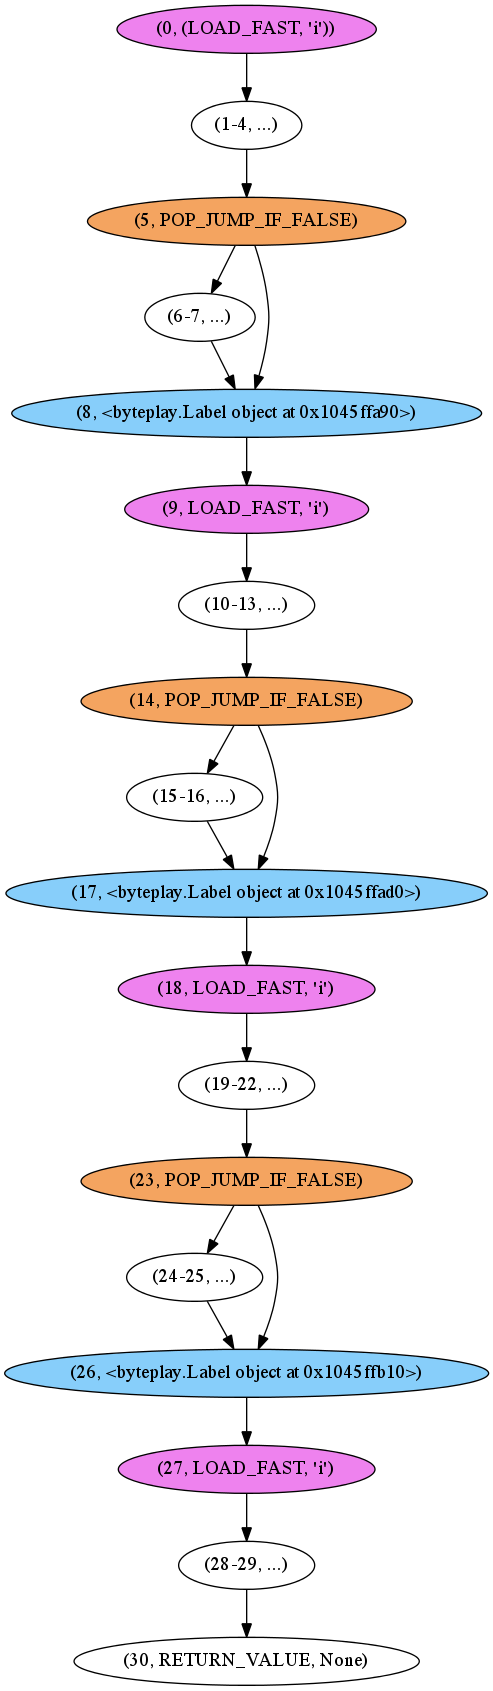
\includegraphics[scale=.39]{img/fizzbuzz.png}
	\caption{FizzBuzz Python module CFG}
	\label{fig:fizzbuzz-cfg}
\end{figure}

\subsubsection{\textsf{Pythoscope}}

\includegraphics[scale=.5]{img/pythoscope-logo.jpg} \textsf{Pythoscope} is an open source unit test generator for Python code, written in Python, licensed under the MIT license. Ideas were contributed by Paul Hildebrandt and Titus Brown, and most of the code so far has been written by Michal Kwiatkowski.

This commandline tool, though extremely easy to setup and use, does not perform the expected automated unit test generation as advertised, but instead only produces a very rudimentary unit test stub below:

\begin{listing}[H]
	\caption{Unit test suite generated by \textsf{Pythoscope}}
	% single
	\begin{minted}[frame=none,linenos,mathescape]{python}
import unittest

class TestTriangle(unittest.TestCase):
    def test___init__(self):
        # triangle = Triangle(a, b, c)
        assert False # TODO: implement your test here

class TestClassifyTriangle(unittest.TestCase):
    def test_classify_triangle(self):
        # self.assertEqual(expected, classify_triangle(triangle))
        assert False # TODO: implement your test here

if __name__ == '__main__':
    unittest.main()
	\end{minted}
	\label{lst:py-triangle-pythoscope}
\end{listing}

\subsubsection{Pytestsgenerator}
This automated unit test case generator creates unit tests for Python modules. The authors Vijakumar and Karthikeyan developed this tool on 32-bit Linux, and it only works for that platform and architecture. Its purpose is to simplify usage of the existing \textsf{PyUnit} framework, and generate logical test cases for classes and methods. \textsf{WxPython} is required as it powers the GUI, but there is also a CLI offered at the same time. The application is packaged for distribution using the \textsf{distutils} module.

According to accompanying documentation, this tool is intended to accomplish the following objectives:
\begin{itemize}
	\item Read a specified python module
	\item List the Classes, Functions and Properties of that module (for the user's selection)
	\item Drill down the Classes for methods and properties
	\item Generate basic set of test cases for each class or method selected
\end{itemize}

The predetermined logic for the test cases to be generated include:
\begin{itemize}
	\item Number of arguments
	\item Valid arguments
	\item Invalid arguments
	\item Custom logic
\end{itemize}

Following is an example demonstration of the software targeting the sample Python module:

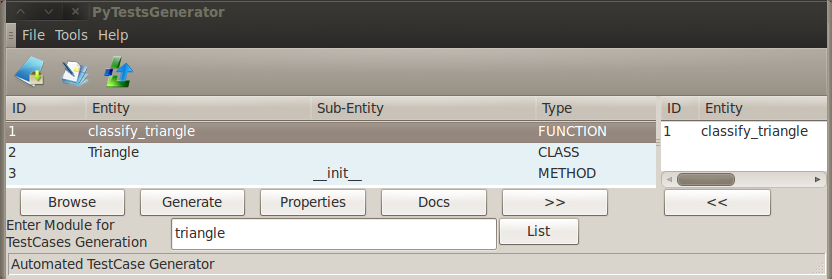
\includegraphics[scale=.51]{img/pytestsgenerator.png}

Using this tool then creates the following unit test stub, included below for comparison:
\begin{listing}
	\caption{Unit test suite generated by \textsf{pytestsgenerator}}
	% single
	\begin{minted}[frame=none,linenos,mathescape]{python}
###Generated using PyTestGenerator
#!/usr/bin/env python

#Format
#test_<Test_Number>_<Entity_Name>[<Arg_Status>]
#	<Predicted_Status>_<Comment>

import unittest
import sys
import triangle

class PyUnitframework(unittest.TestCase):
	'''Test Cases generated for triangle module'''

if __name__=="__main__":
	testlist=unittest.TestSuite()
	testlist.addTest(unittest.makeSuite(PyUnitframework))
	result = unittest.TextTestRunner(verbosity=2) \
		.run(testlist)
	if not result.wasSuccessful():
		sys.exit(1)
	sys.exit(0)
	\end{minted}
	\label{lst:py-triangle-pytestsgenerator}
\end{listing}

As evident from the code snippets of the generated unit test stubs, both these tools are still fairly inadequate for automatically discovering unit tests for arbitrary Python programs.

%%%%%%%%%%%%%%%%%%%%%%%%%%%%%%%%%%%%%%%%%%%%%%%%%%%%%%%%%%%%%%%%%%%%%%%%%%%%%%%%%%%%%%%
\section{The Python programming language}
\label{sect:bkgrd-python}

Python is a general-purpose, multi-paradigm (imperative/object-oriented/functional programming styles), high-level programming language, whose design philosophy emphasises code readability. It features a fully dynamic type system and automatic memory management. Its syntax is said to be clear and expressive. It is often used as a scripting language, but can also be applied in a wide range of non-scripting contexts, popular with the numeric and scientific community.

Python has a large and comprehensive standard library. Using third-party tools, Python code can be packaged into standalone executable programs. Python interpreters are available for many operating systems. Its reference implementation is CPython.

Unlike statically typed languages, Python features a number of expected runtime characteristics unique to the class of dynamic languages: dynamic typing, interpretation (seamless source code compilation when needed), introspection/reflection and runtime modification.

\subsection{Dynamic typing}
The beauty of dynamic languages is dynamic typing, otherwise also expressed as `duck typing', meaning objects are described by what they can or cannot do, i.e. by the methods it responds to at runtime, instead of being associated to a specific type.

Pythonic programming style that determines an object's type by inspection of its method or attribute signature rather than by explicit relationship to some type object. By emphasising interfaces rather than specific types, well-designed code improves its flexibility by allowing polymorphic substitution. Duck-typing avoids tests using \pyth{type()} or \pyth{isinstance()}. Instead, it typically employs the EAFP (Easier to Ask Forgiveness than Permission) style of programming.

Values possess types instead of variables, and often the type of objects sent in as function arguments or produced in method invocations as return results are not strictly checked against.

When code is executed, the execution environment need not care what type an object has, only if it implements the methods that are called on it. This makes Python an attractive prototyping language for this study, yet at the same time poses complications (difficulty in identifying input data for method invocations, because arguments can be used in different ways) in searching for adequate test cases, due to its dynamic nature. It is therefore essential to limit the size of the search space to be considered to maintain a reasonable execution time for generating tests.

\subsection{Introspection/reflection}
This makes it much easier to collect relevant information about classes and methods at runtime. It is not only possible to query for the availability of methods during object creation as well as the code implementation behind it, but also to search for methods that may change the internal state of an object as well as identifying their arguments.

\subsection{Runtime modification}
Runtime modification is a central characteristic of dynamic languages. A type, value or code object can typically be altered (changed/added) during runtime in a dynamic language (actual allowed behaviours vary between languages). This means generating new objects from a runtime definition, creation and loading of entire new system modules, or changing the inheritance or type tree, thus changing the way existing types behave, especially with respect to method invocations.

The use of this feature usually only exists in a small percentage of code like creating this automated unit test generator, whilst the rest is designed in a more traditional manner. For these reason, the testing of code including the \pyth{exec()} or \pyth{eval()} keywords are excluded from this study.
%%%%%%%%%%%%%%%%%%%%%%%%%%%%%%%%%%%%%%%%%%%%%%%%%%%%%%%%%%%%%%%%%%%%%%%%%%%%%%%%%%%%%%%

\section{Challenges}
\label{sect:challenges}
There are several facets of complexity to this problem, which this work hopes to tackle.

\subsection{Function argument instantiation}
Function arguments can range from basic primitive types, to dynamic data structures like lists, maps, and trees, to objects. Depending on available resources, scope for this project might be restricted to supporting only numeric types and objects.

These classes of values present distinct challenges, when they appear as input arguments to functions being tested. Intuitively, the search space for a primitive integer type, for instance, extends in one direction towards positive infinity if unsigned, and in both directions if signed. However, for complex data structures like trees, the notion of infinity manifests itself via nesting as well.

Even the usage of basic types may become quite complex, especially when there is only a small solution space, in which a certain condition can be satisfied. This might extend beyond single arguments to a combination of them, and this is exacerbated when arguments can depend on other values, or previous argument values.

This is especially applicable not only to class constructors, when creating appropriate objects, but also in automatically generating initial function input arguments.

It is vital to ensure that an exhaustive enumeration of the search space in search of 
pathological test cases is not performed, because there would quickly be an exponential blow up, especially in functions with multiple input arguments, as well as being inefficient, due to the side effect of generating many redundant or subsumed test cases.

There are several possible ways to conduct the search for such corner cases. Previous algorithms range from \naive systematic enumeration of all possible values to variants of random testing.

Another complexity factor is added when there are dependency between functions, arising from the argument to one having to be constructed by the other. This naturally enforces a fixed sequence in which to order the function invocations and entails that the automated unit test generation framework respect this ordering so as to create significant test cases.

Therefore, the task here is to come up with a more efficient way of prioritising pathological boundary parameter value generation, under real time and space constraints. Some leading intuition follows.
%%%%%%%%%%%%%%%%%%%%%%%%%%%%%%%%%%%%%%%%%%%%%%%%%%%%%%%%%%%%%%%%%%%%%%%%%%%%%%%%%%%%%%%
\subsubsection{Lazy instantiation}
It might be reasonable to begin with ``lazy instantiation" \cite{Allwood2011}, where dummy \textsf{null}ified objects are passed in initially. Test data is only generated for return values when the methods on them are actually invoked. This supposes multiple runs through the same code block, and using feedback from previous iteration to direct future execution.

As for implementing the idea of \emph{lazy instantiation}, \textsc{Irulan} \cite{Allwood2011} is the canonical reference tool written to demonstrate this concept in Haskell. This project intends to investigate further into the feasibility of applying this concept to Python.

A sample execution to discover errors in the following code snippet:

\begin{lstlisting}[language=HaskellUlisses,frame=single]
module IntTreeExample where
data IntTree
	= Leaf
	| Branch IntTree Int IntTree
insert :: Int -> IntTree -> IntTree
insert n Leaf = Branch Leaf n Leaf
insert n (Branch left x right)
	| n < x = Branch (insert n left) x right
	| n > x = Branch left x (insert n right)
\end{lstlisting}
\clearpage
produces the following output:
\begin{lstlisting}[language=HaskellUlisses,frame=single]
$ irulan --ints='[0,1]' --enable-case-statements -a --maximumRuntime=1 source IntTreeExample
...
insert 1 (Branch ? 1 ?1) ==> !
IntTreeExample.hs:(8,0)-(11,41): Non-exhaustive patterns in function insert
insert 0 (Branch ? 0 ?1) ==> !
IntTreeExample.hs:(8,0)-(11,41): Non-exhaustive patterns in function insert
case insert 0 (Branch (Branch ? 0 ?1) 1 ?2) of
Branch x _ _ -> x ==> !
IntTreeExample.hs:(8,0)-(11,41): Non-exhaustive patterns in function insert
case case insert 0 (Branch (Branch (Branch ? 0 ?1) 1 ?2) 1 ?3) of
Branch x _ _ -> x of
Branch x _ _ -> x ==> !
IntTreeExample.hs:(8,0)-(11,41): Non-exhaustive patterns in function insert
...
\end{lstlisting}

\subsubsection{Runtime in-memory manipulation}
It is also envisioned that the dynamic language features of Python be exploited in order to rapidly generate useful test data. One idea is to manipulate and observe the behaviour of code blocks in memory at runtime, by monkeypatching or hotswapping code under test (CUT) for stubs, but with a hook to log incoming parameters during a sample execution, in order to determine their initial starting range \& types.

On a related note, a cross-cutting concern such as logging may be implemented using the concept of Aspect Oriented Programming (AOP), with tools like \textsf{pytilities}, \textsf{Aspyct}, \textsf{aspects.py} or \textsf{PythonDecoratorLibrary}.

\subsubsection{Random testing}
Apart from random testing with feedback RANDOOP \cite{Pacheco2007}, and preferring configuration diversity over a single optimal test configuration in Swarm testing \cite{AlexGroceSep2011}, another suggestion is to inspect stack frames of previous executions to grasp a better initial starting point for generating parameters.
%%%%%%%%%%%%%%%%%%%%%%%%%%%%%%%%%%%%%%%%%%%%%%%%%%%%%%%%%%%%%%%%%%%%%%%%%%%%%%%%%%%%%%%
\subsection{Optimising search space coverage}
The suggestion to parallelise the search space for interesting values over the entire range of integers for example, is to use the General Purpose Graphics Processing Unit (GPGPU) toolkit like Nvidia's CUDA or HADOOP cluster, of which its feasibility remains to be determined.

Alternatively, parallelism has already been achieved \cite{Pargas99}, by running multiple processes simultaneously on a network of workstations or on a single multi-core processor, with a user-determined numerical parameter. In that experiment, each process running on separate workstations communicated to maintain synchronisation via a software facility.

The benefit is clear: reduction in execution time by a factor of the number of parallel processes. This seems possible, given a way to partition the test case generation workload into several balanced independent components, according to the available resources.
%%%%%%%%%%%%%%%%%%%%%%%%%%%%%%%%%%%%%%%%%%%%%%%%%%%%%%%%%%%%%%%%%%%%%%%%%%%%%%%%%%%%%%%
\subsection{Testing a dynamically typed language}
Much of the body of work in the software testing community concerns testing against static languages, rather than dynamic languages, or even Python in particular.

Dynamically typed languages are characterised by values having types, but not variables, hence a variable can refer to a value of any type, which can possibly cause test data generation to become more complicated. Python therefore heavily employs duck typing, to determine an object's type by inspection of its method or attribute signatures.

Tools arising from research efforts into testing for static languages lacks adequate support for code written in dynamic languages, including typical features such as \texttt{eval()}, closure, continuations, functional programming constructs, and macros, thus this paper aims to look into this further, in the context of Python.
%%%%%%%%%%%%%%%%%%%%%%%%%%%%%%%%%%%%%%%%%%%%%%%%%%%%%%%%%%%%%%%%%%%%%%%%%%%%%%%%%%%%%%%
\subsection{Non-terminating program executions}
Another difficulty associated with this problem domain is detecting infinite executions when generating test code. This can be most commonly attributed to (the error of) infinite loops present, which may even be nested. It is impossible to detect all kinds of loops fully automatically, but many such can \cite{Tahbildar}. An immediate solution is to implement timeouts, with custom duration according to CUT. Early detection so as to improve efficiency is difficult.
%%%%%%%%%%%%%%%%%%%%%%%%%%%%%%%%%%%%%%%%%%%%%%%%%%%%%%%%%%%%%%%%%%%%%%%%%%%%%%%%%%%%%%%
\subsection{Early detection of path infeasibility}
The paper \cite{Tahbildar} claims one of the most time consuming task of automatic test data generation is the detection of infeasible path after execution of many statements. Hence, backtracking on path predicates \cite{Korel1990}, satisfiability of a set of symbolic constraints \cite{ZhangW01}, selectively exploring a subset of "best" paths \cite{Prather1987} are some of the past attempts at solving this issue. This is a major problem of test data generation based on actual value, incurring both costly and unnecessary computation.
%%%%%%%%%%%%%%%%%%%%%%%%%%%%%%%%%%%%%%%%%%%%%%%%%%%%%%%%%%%%%%%%%%%%%%%%%%%%%%%%%%%%%%%
\subsection{Improving code coverage}
Achieving consistently high code coverage over a wide range of programs (not to mention running within reasonable time and space) via generated test cases ultimately defines the extent of success of this project. This allows for effective fault detection, which may be of different types. An alternative measurement of code coverage improvement involves identifying error prone regions of code where more rigorous testing would prove beneficial \cite{Ntafos1988} \cite{InceDC1987}. There already exists other empirical studies for code coverage in different test data generation algorithms documented, providing some competitive standards to match up to \cite{Han2008} \cite{Rothermel99testcase} \cite{Lakhotia2009}.
%%%%%%%%%%%%%%%%%%%%%%%%%%%%%%%%%%%%%%%%%%%%%%%%%%%%%%%%%%%%%%%%%%%%%%%%%%%%%%%%%%%%%%%
\section{Summary}
In this chapter, the relevant background literature and theory to understand this project has been explained in sufficient detail. The next chapter presents the theoretical foundation underpinning this project's contributions to the field of software testing, including the problem specification, approach taken, and algorithms and techniques used, to name a few.
%%%%%%%%%%%%%%%%%%%%%%%%%%%%%%%%%%%%%%%%%%%%%%%%%%%%%%%%%%%%%%%%%%%%%%%%%%%%%%%%%%%%%%%
\chapter{Contributions}
\label{ch:contrib}
\textcolor{red}{<Missing introductory paragraph>}
\section{Specification}
The strategy in this project emphasises dynamic test data generation, where intermediate runtime data is gathered, represented in some suitable form, and used to guide subsequent testing iterations.

Our strategy assumes that the CUT is not obsfucated, so reverse engineering and code reconstruction lies out of the scope of this investigation.

Moreover, we are dealing only with Object Oriented (OO) style Python programs, i.e. those involving classes and objects.

As an simplifying assumption, the CUT here is limited to contain at most one program entry point. If the CUT is found not to contain a main entry point, then tests are generated for the individual classes and functions separately, as discovered by the runtime engine.

In addition, test cases should be generated without requiring any user input.

SUT is modelled as a combination of a main program entry point, top level functions, together with classes containing fields and methods. Functions are restricted to entities which receive some input arguments, uses some or all of these in its body for computation, and finally returns some of these values.

The scope is also restricted to exclude test data generation to cover branches with string predicates, for which another study addresses string equality, string ordering and regular expression matching \cite{Alshraideh2006}.

\subsection*{Example}
Given a basic standard complete implementation of class \textsf{LinkedList}, with a sample of prototype of method signatures detailed below:

\lstset{language=Python}          % Set your language
\begin{lstlisting}[frame=single]  % Start your code-block

def add(self, isAdd):
def size(self):
...
\end{lstlisting}

This project aims to then create the following test suite to validate its behaviour:

\begin{lstlisting}[frame=single]  % Start your code-block

Test #1:
	l = LinkedList()
	assert (l.size == 0)
Test #2:
	l = LinkedList()
	l.add(true)
	assert (l.size == 1)
Test #3:
	l = LinkedList()
	l.add(true)
	i = l.iterator
	assert (i.hasNext)
\end{lstlisting}

These generated test cases within the suite should ideally be as close to natural language as possible, as a project extension.
%%%%%%%%%%%%%%%%%%%%%%%%%%%%%%%%%%%%%%%%%%%%%%%%%%%%%%%%%%%%%%%%%%%%%%%%%%%%%%%%%%%%%%%
\section{Approach}
Some notable aspects of the proposed solution:
\begin{enumerate}[i.]
	\item developed incrementally
	\item bytecode inspection
	\item runtime construction of control flow graph (CFG) / control dependence graph (CDG)
	\item runtime code manipulation
	\item introspection \& reflection
	\item Python 2.7.x module
	\item target Mac OS X / Ubuntu Linux
\end{enumerate}

A preliminary sample of the bytecode investigation for simple language constructs can be found in the Appendix section of this paper.

The key deliverable from this project will be unit test suites, in terms of a language-neutral Domain Specific Language (DSL), or Javascript Object Notation (JSON), consisting of various assertions, capture expressions, and value assignments. This affords flexibility in later system extensions to target other dynamic programming languages.

An API may be exposed if there are reusable components, eg. algorithms, developed in this tool. It is also planned to provide visualisation of this process, in the form of a GUI frontend, powered by wxPython/GTK.

The resulting end product can be applied to regression testing as well, to report changes in behaviour across different versions, as software evolves over time.

\section*{Available tools}
Detailed below as follows are the selection of Python resources for various purposes:
\begin{enumerate}[i.]
	% @ http://nedbatchelder.com/text/python-parsers.html
	\item \emph{\href{http://wiki.python.org/moin/LanguageParsing}{parsing modules}} - ANTLR, PyParsing, Ply (Python Lex-Yacc), Spark, parcon, RP, LEPL, 
	\item \emph{measuring code coverage} - coverage.py, figleaf, trace2html
	\item \emph{\href{http://wiki.python.org/moin/PythonTestingToolsTaxonomy}{unit testing}} - (X)PyUnit, TestOOB, unittest, nose, py.test, peckcheck
	\item \emph{mutation testing} - Pester
	\item \emph{bytecode inspection \& manipulation} - Decompyle (2.3), UnPyc (2.5,2.6), pyREtic (in memory RE)
	\item \emph{Python DSL} - Konira
	\item \emph{syntax highlighting} - Pygments
	\item \emph{CUDA Python bindings}
	\item \emph{Python language reference} - Grammar
	\item \emph{documentation} - epydoc
	\item \emph{Alternative implementations} - PyPy, Unladen Swallow
	\item \emph{fuzzing tools?}
	\item \emph{supporting tools} - virtualenv/pip
\end{enumerate}
%%%%%%%%%%%%%%%%%%%%%%%%%%%%%%%%%%%%%%%%%%%%%%%%%%%%%%%%%%%%%%%%%%%%%%%%%%%%%%%%%%%%%%%
\section{Algorithm}

Generating complex input data

	Dynamic data structures, like lists and binary trees, can be divided into four possible categories\cite{Zhao2007}:
		- assignment
		- creation
		- deletion
		- comparison statements
			The comparison is further categorised into equal and unequal conditions
	\cite {}

\subsection{The test data generation algorithm}

	\subsubsection{Step 1: Construction of the CFG}
	\subsubsection{Step 2: Initial path selection}
	\subsubsection{Step 3: Derivation of linear constraints}
	...

\subsection{Examples}
A simple example shall be provided to illustrate the basic approach of test data generation. Consider the program of Figure XX which is supposed to YY.
Given the following path P ..., the goal of the test data generation is to find a program input x which will cause P to be traversed.

The program is executed on this input, and the following successful subpath $P_1$ is traversed ...

%%%%%%%%%%%%%%%%%%%%%%%%%%%%%%%%%%%%%%%%%%%%%%%%%%%%%%%%%%%%%%%%%%%%%%%%%%%%%%%%%%%%%%%
\section{Summary}
In this chapter, the current research work has been highlighted. In order to demonstrate the idea of automated lazy testing in Python, an example usage of the tool is provided, using the ideas found in this chapter. The structure of this tool, and the examples, is the subject of the next chapter.
%%%%%%%%%%%%%%%%%%%%%%%%%%%%%%%%%%%%%%%%%%%%%%%%%%%%%%%%%%%%%%%%%%%%%%%%%%%%%%%%%%%%%%%
\chapter{\textsc{Splat}}
\label{ch:splat}

In this section, the tool \textsc{Splat} is introduced, together with its various components.

\section{Architecture}
The software design architecture is outlined below:
\begin{center}
\begin{tikzpicture}
  [node distance=1cm,
  start chain=going below]
  % nodes
  \node[value] (progin) {Unobsfucated Python bytecode input};
  \node[component] (proganal) {Program analyser};
  \begin{scope}[start branch=zero,]
	  \node (paramiface) [text width=2cm,align=right,on chain=going left] {Parameter interface};
	  \begin{scope}[start branch=one,]
    	  \node (codeblock) [text width=2cm,align=right,on chain=going above] {Basic code blocks};
	  \end{scope}
	  \begin{scope}[start branch=two,]
    	  \node (normconstraint) [text width=2cm,align=right,on chain=going below] {Normalised constraints};
	  \end{scope}
  \end{scope}
  \node[component,join] (codeinst) {Code instrumentor};
  \node[component,join] (rt) {Runtime engine};    
  \begin{scope}[start branch=feedback,]
	  \node[component,on chain=going right,yshift=-1.2cm] (datastore) {Datastore};
	  \node[component,join,on chain=going above] (testdatagen) {Test data generator};
  \end{scope}
  \node[component,join] (testgen) {Test case generator};
  \node[value] (testout) {Assertions-based unit test DSL output}; 
  % edges
  \draw[->, thick, dashed] (progin.south) -> (proganal.north);
  \draw[->, thick, dashed] (testgen.south) -> (testout.north);

  \draw[->, thick] (proganal.west) -> (codeblock.east);
  \draw[->, thick] (proganal.west) -> (paramiface.east);
  \draw[->, thick] (proganal.west) -> (normconstraint.east);
  \draw[->, thick] (testdatagen.west) -> (rt.north east);
  \draw[->, thick] (rt.south east) -> (datastore.west);
  \draw[category,decoration={brace}] let \p1=(proganal.north), \p2=(proganal.south) in
    ($(2.2, \y1)$) -- ($(2.2, \y2)$) node[catlabel] {
	    \makecell[l]{Extracts code-specific\\information}
	};
  \draw[category,decoration={brace}] let \p1=(testdatagen.north east), \p2=(datastore.south east) in
    ($(7.4, \y1)$) -- ($(7.4, \y2)$) node[catlabel,text width=2cm] {Feedback mechanism};
  \draw[category] let
    \p1=(datastore.south east), \p2=(datastore.south west) in
    ($(\x1,\y1-.4em)$) -- ($(\x2,\y2-.4em)$) node[below, midway] {
    	\makecell[l]{- runtime state\\- program abstraction CFG}
    };
\end{tikzpicture}
\end{center}
%%%%%%%%%%%%%%%%%%%%%%%%%%%%%%%%%%%%%%%%%%%%%%%%%%%%%%%%%%%%%%%%%%%%%%%%%%%%%%%%%%%%%%%
Test data generation uses the branch coverage algorithm to select a path that may reach the targeted branch and obtains constraint information for the selected path to then generate the test data inputs for the resulting test cases. This only applies to the relevant 'control points', i.e. absolute and relative jumps to labels in bytecode, where the conditional is somewhat dependent on the incoming function arguments.

%%%%%%%%%%%%%%%%%%%%%%%%%%%%%%%%%%%%%%%%%%%%%%%%%%%%%%%%%%%%%%%%%%%%%%%%%%%%%%%%%%%%%%%
\section{Examples}
...
%%%%%%%%%%%%%%%%%%%%%%%%%%%%%%%%%%%%%%%%%%%%%%%%%%%%%%%%%%%%%%%%%%%%%%%%%%%%%%%%%%%%%%%
\section{Summary}
In this chapter, the working automated testing tool has been shown, but exactly how well does it actually perform against current standards? This notion will be made more precise, both quantitatively and qualitatively, in the next chapter focusing on the evaluation of this work.
%%%%%%%%%%%%%%%%%%%%%%%%%%%%%%%%%%%%%%%%%%%%%%%%%%%%%%%%%%%%%%%%%%%%%%%%%%%%%%%%%%%%%%%
\chapter{Evaluation}
\label{ch:eval}
\section{Experiment}
Experimental evaluation entails the following:
\begin{enumerate}[i.]
	\item comparison with existing work, eg. Pythoscope (2010), PyTestsGenerator (2009)
	\item benchmark against popular Python libraries - python-graph, and Python module implementations of famous algorithms
	\item measure quality of test cases generated using metrics - bugs and crash discovery (pathological inputs)	
\end{enumerate}

\subsection{Evaluation criteria}
An explanation of and in depth discussion into the adequacy of the different strands of test code coverage criteria and how the various metrics established are used to grade the effectiveness of this tool against the benchmark suite in automatically generating unit test data forms the theme of this section.

Throughout this section, P is a program under test and C is a selected test coverage criteria. T is a set of test data which satisfies 100\% of test requirements of C for a P. M is a test data generation method and T' is a set of test data found by M for a P and C.

\subsubsection{Code coverage}
Test coverage criteria serve as a means to explicitly state the extent to which a test requirement (i.e. statements, branches, or conditions) has been tested.

The effectiveness of test data generation can be measured using \emph{branch coverage} as one of the criteria, by ensuring that all possible branches in valid program execution paths are selected, reached and traversed, when exercised by the generated unit test suite.
...(statement, path, branch) coverage 

\subsubsection{Linear Code Sequence And Jump (LCSAJ)}
Linear code sequence and jump (LCSAJ) is a software analysis method used to identify structural units in code under test. Its primary use is with dynamic software analysis to help answer the question ``How much testing is enough?". Dynamic software analysis is used to measure the quality and efficacy of software test data, where the quantification is performed in terms of structural units of the code under test. When used to quantify the structural units exercised by a given set of test data, dynamic analysis is also referred to.

\subsubsection{Performance}
The performance of a test data generation method should be viewed in two different aspects, the first of which is the \textbf{effectiveness} of a test data generator - the fraction of test requirements covered by T', ignoring unreachable branches, occurring likely due to logical program errors.

The other aspect measured is the \textbf{efficiency} of a test data generation method in terms of its space and runtime complexity. Space efficiency is affected by the amount of information stored during the process of gathering test data for generation. In general, plenty of space is required for the static approach, especially symbolic execution-based methods, whereas the dynamic approach requires relatively less space in comparison, because of the difference between static analysis information and runtime data.

In contrast, the static approach is more economical than the dynamic approach as far as time requirements are concerned. While the dynamic approach needs many iterations, and a single execution of the SUT is the most significant computational cost, the solution can be derived quickly in a single pass in the static approach, neglecting the fact that obtaining a solution from the set of algebraic expressions could result in a complex computation.

\subsubsection{Quality of test data}
The quality of test data is related to how many faults are detected by T'. If a set of test data $T'_1$ can reveal more faults in P than the other set of test data $T'_2$ for a given M and C, $T'_1$ is of a better quality than $T'_2$. Therefore, the quality of test data generated is measured by seeding errors into P via a mutation testing technique.

\paragraph{Mutation testing}
Mutation testing is a fault-based method of software testing designed to create effective test data. It works by randomly modifying programs source code or bytecode in slight but critical ways. Any tests which pass after code has been mutated are considered defective, called as `mutations'.

This procedure is established on well-defined mutation operators that either mimic typical software or human error, and supposedly leads to the creation of more valuable unit tests.

Its purpose is to evaluate the effectiveness of the automatic test data generation strategy, especially when it comes down to the `weaker' parts of code that are seldom or never accessed during normal program execution, and so probably less extensively tested.

The basic steps involved here are as follows:
\begin{itemize}
	\item begin with the test suite generated automatically, and the one written manually by hand.
	\item once verified that both pass on a given piece of program code, apply a mutation to the bytecode of this SUT.
	\item the extent of mutation can vary, from the very elementary substitution of a logical operator with its complement. For instance, \texttt{==} can be transformed into \texttt{!=}, while \texttt{<} would turn into \texttt{>=}.
	\item the more complex operations would be as drastic as reordering code execution or removing parts of code completely.
	\item however, mutations of this degree frequently cause compiler errors, defeating the purpose of this evaluation altogether, so it is often more advisable to perform the simpler mutations mentioned instead.
	\item after this, both the original test suites are re-run against this program.
	\item if the test suites were effective, they should now be expected to fail in covering the mutated program.
	\item otherwise the test is not well written, as it is creating false positives, and needs to be revisited.
	\item of course, a scoring metric can be invented to denote partial success in generating unit tests, should it be the case that only some of the tests pass on the mutant program.
\end{itemize}

\subsubsection{Generality}
The generality of a test data generation method indicates its ability to function in a wide selection and practical range of situations. Ideally, the test data generation method should function in the presence of arbitrarily complex programs.

The less the test data generation method is restricted by language constructs and target languages in which the program is written, the more generally applicable the test data generation method is, which is why this project sets out to generate unit tests in a language-neutral format like JSON.

The test data generation method should work on the complex program to be used in practice. The coverage rate in P by T' according to the complexity of each program needs to be examined. If a test data generator covers all target branches on the complex program, it is said to be generally applicable, which is the desired characteristic.

\subsection{Selection of programs}
Before preparation for experimentation, candidate programs have to be select as unit test data generation targets. The features used are loops, arrays, non-linear predicates and module calls, input data type - numeric: integer or floating point, or objects, and the complexity of a program, referring to the cyclomatic complexity metric as well as nesting (of conditionals) and condition complexity (number of boolean expressions within a conditional).

Cyclomatic complexity (CC) directly measures the number of linearly independent paths through program code, and is computing using its CFG. It is more precisely defined by the following equation:
$$
	M = E - N + 2P
$$
where M is the cyclomatic complexity, E is the number of edges in the flowgraph, N the number of nodes of the graph, and P is the number of connected components (exit nodes).

\subsection{Coverage results}

\subsection{Errors found}

% profiling test targets - SLoC, CC
% project/method coverage%;time SPLAT vs. Random Testing
% graph of code coverage over #iterations/time
% Evaluate choices of unit testing frameworks, unittest, py.test, PyUnit...

%%%%%%%%%%%%%%%%%%%%%%%%%%%%%%%%%%%%%%%%%%%%%%%%%%%%%%%%%%%%%%%%%%%%%%%%%%%%%%%%%%%%%%%
\section{Summary}
The results achieved and comparison of desired outcomes with original expectations are examined here in this chapter. To finish off, the next chapter summarises this entire paper and hints at what might be possible future research directions in this area of automated software testing.
%%%%%%%%%%%%%%%%%%%%%%%%%%%%%%%%%%%%%%%%%%%%%%%%%%%%%%%%%%%%%%%%%%%%%%%%%%%%%%%%%%%%%%%
\chapter{Conclusion \& Future Work}
\label{ch:conclusion}
The following is a simple non-exhaustive enumeration of 'could-haves', if time permits:
\begin{itemize}
	\item An API to allow for other developers to contribute to the development of this tool, and make use of the algorithms contained therein in isolation
	\item Comprehensive documentation on the internal workings and usage of the tool, with examples provided as well
	\item Visualisation for the tool via a user-friendly GUI frontend, powered by wxPython/GTK
	\item Improve sophistication of the tool to generate more robust and thorough tests, test code containing more complex interaction of language constructs, or deal with new language features in Py3k
	\item Optimise efficiency of tool in test generation, by compiling on a faster Python implementation for instance, or scaling parallel search
	\item Benchmark tool across a wider range of different Python frameworks and libraries
	\item Explore other techniques and algorithms to attempt to improve overall test code coverage
\end{itemize}
%%%%%%%%%%%%%%%%%%%%%%%%%%%%%%%%%%%%%%%%%%%%%%%%%%%%%%%%%%%%%%%%%%%%%%%%%%%%%%%%%%%%%%%
% Bibliography
%%%%%%%%%%%%%%%%%%%%%%%%%%%%%%%%%%%%%%%%%%%%%%%%%%%%%%%%%%%%%%%%%%%%%%%%%%%%%%%%%%%%%%%
\bibliographystyle{alpha}
\nocite{*}
\bibliography{FYP}\addcontentsline{toc}{chapter}{Bibliography}
%%%%%%%%%%%%%%%%%%%%%%%%%%%%%%%%%%%%%%%%%%%%%%%%%%%%%%%%%%%%%%%%%%%%%%%%%%%%%%%%%%%%%%%
\end{document}
